\documentclass[11pt,a4paper]{article}

\usepackage[margin=2.15cm]{geometry}
\usepackage{graphicx}
\usepackage{booktabs}
\usepackage{amsmath}
\usepackage[round]{natbib}
\usepackage[hidelinks]{hyperref}
\usepackage{microtype}
\usepackage{caption}
\captionsetup{font=small,labelfont=bf}
\setlength{\bibsep}{2pt}
\setlength{\textfloatsep}{9pt plus 2pt minus 2pt}
\setlength{\intextsep}{9pt plus 2pt minus 2pt}
\setlength{\abovecaptionskip}{5pt}

\title{\Large\textbf{Emergent Tipping Points in AI Labour Markets:\\
Design and Outcomes of a Task-Based Agent-Based Simulator}}
\author{Johannes Meier}
\date{July 2026}

\begin{document}
\maketitle

\begin{abstract}
\noindent
How artificial intelligence reshapes labour markets depends on interactions between
firm-level adoption decisions and worker-level reallocation that aggregate models
struggle to represent without assuming their conclusions. This paper describes the
design of an open, task-based agent-based model (ABM) in which roughly 5{,}000 workers
and 400 firms interact monthly: firms adopt AI task-by-task when quality-adjusted AI
costs undercut wages, amplified by sectoral imitation and heterogeneous organizational
hurdles, while displaced workers search, bargain, and retrain across an occupation space
whose geometry derives from task-content similarity. No functional form for diffusion is
imposed; adoption S-curves, displacement waves, wage scarring, and Beveridge-curve
loops all emerge from micro-interactions. A no-AI baseline is calibrated to empirical
labour-flow anchors and locked as an automated test gate before any AI mechanism is
introduced. Simulation experiments show that a fast-takeoff scenario raises output by
roughly 80\% while labour-market distress climbs from an early displacement spike near
20\% of the workforce toward a third under sustained automation, that median wages
halve while within-labour dispersion \emph{compresses} toward the benefit
floor---shifting the surplus toward firms rather than spreading it among
workers---that in knowledge occupations split into junior and senior variants the
pyramidal apprenticeship structure \emph{inverts}, with the junior rung eliminated
within years while augmented senior employment persists---and that canonical policy
levers are strikingly non-robust:
unemployment-benefit generosity lowers median peak distress in the final specification
yet worsens a minority of seeds and reversed sign under an earlier revision of the
demand block; employment protection leaves median peak distress essentially unchanged
while flipping sign seed-by-seed; only the efficiency of reallocation itself delivers a
consistent median improvement. The model
ships as an interactive web application with Monte Carlo uncertainty quantification and
full seed-level reproducibility. We close with an agenda for empirical curation,
mechanism extensions, and validation.
\end{abstract}

\begin{figure}[b!]
\centering
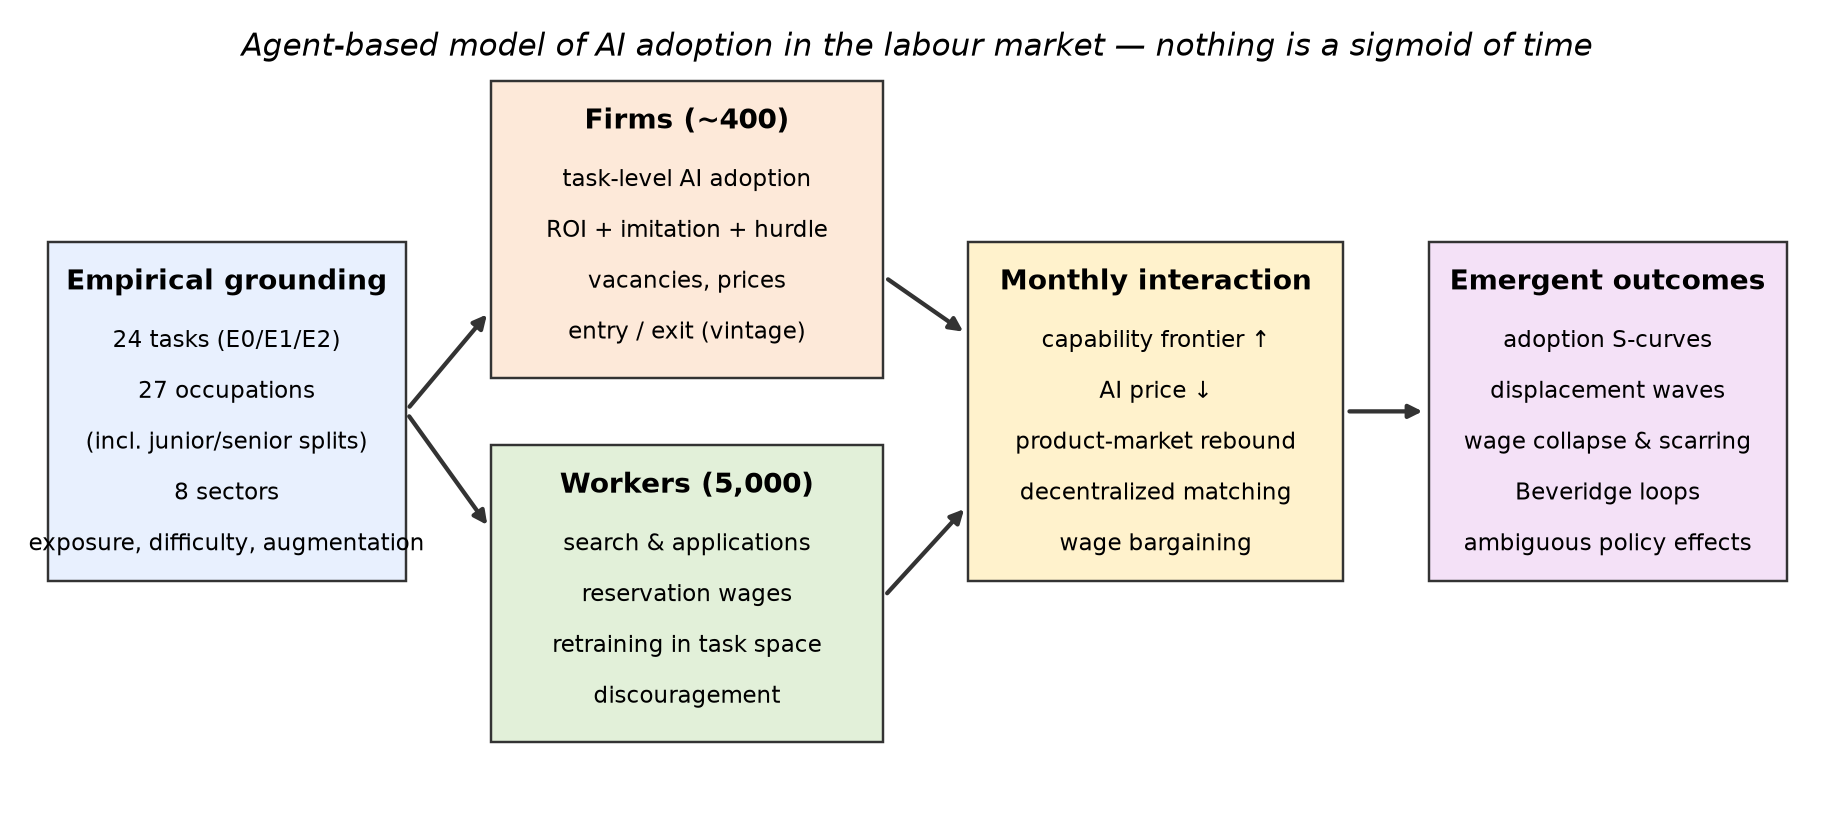
\includegraphics[width=0.94\textwidth]{figures/fig_schematic.png}
\caption{Graphical abstract. Empirically grounded tasks, occupations, and sectors
parameterize heterogeneous firm and worker agents whose monthly interactions on product
and labour markets generate emergent macro-level dynamics. No sigmoid of time appears
anywhere in the model code.}
\label{fig:schematic}
\end{figure}

\section{Introduction}

The question of how artificial intelligence will transform employment has moved from
speculative long-range forecasting \citep{frey2017future} to an urgent empirical and
policy debate, as large language models demonstrably perform a substantial share of
economically relevant tasks \citep{eloundou2024gpts, noy2023experimental,
brynjolfsson2025generative}. The dominant analytical tradition treats this question at
the aggregate level: task-based production frameworks decompose occupations into
automatable and complementary components \citep{autor2003skill, acemoglu2018race,
acemoglu2019automation}, and scenario analyses trace out macroeconomic paths under
assumptions about the speed and breadth of automation \citep{korinek2024scenarios,
korinek2024policy}. These approaches are powerful, but they share a structural
limitation: the dynamics of interest---the timing of adoption take-off, the depth of
transitional unemployment, the distribution of wage losses---are typically encoded
directly in functional forms such as logistic diffusion curves and aggregate matching
functions. The model then illustrates its assumptions rather than testing whether the
posited dynamics can arise from plausible micro-behaviour.

This paper takes the complementary, generative route \citep{epstein1996growing,
tesfatsion2006ace}. We present the design and first results of an agent-based model
(ABM) in which the units of analysis are the actual decision-makers: firms that weigh
the return on automating specific tasks against adjustment costs and organizational
inertia, and workers who search for jobs, form reservation wages, and retrain toward
occupations whose task content resembles what they already know. The model's central
discipline is that \emph{nothing tips by construction}. Adoption accelerates only if
falling AI prices, advancing capability, heterogeneous adoption hurdles, and imitation
externalities jointly produce acceleration; unemployment spikes only if displacement
outruns a decentralized matching process; inequality rises only if automation reprices
some workers' marginal products relative to others.

The contribution is threefold. First, we describe a compact, fully reproducible model
architecture---roughly 930 lines of tested Python built on the Mesa~3 framework
\citep{kazil2020mesa, terhoeven2025mesa}---that connects the task-exposure measurement
literature \citep{eloundou2024gpts, felten2021occupational, webb2020impact,
handa2025economic} to search-and-matching labour-market dynamics
\citep{mortensen1994job, pissarides2000equilibrium} inside a single computational
laboratory. Second, we introduce a calibration-gate methodology: the no-AI baseline is
tuned to empirical labour-flow anchors and then \emph{locked as an automated test suite}
that every subsequent mechanism must keep green, which guards against the parameter
drift that afflicts macro ABMs \citep{fagiolo2017macro}. Third, we report emergent
outcomes with direct policy relevance, including a result that aggregate treatments
cannot even express: the transitional-distress effects of unemployment benefits and
employment protection are seed- and specification-dependent, with medians, dispersions,
and even signs that shift across replications and model revisions, while only the
efficiency of reallocation itself is consistently beneficial.

\section{Related work}

Task-based models of automation originate with \citet{autor2003skill} and were
generalized by \citet{acemoglu2018race, acemoglu2019automation}, who emphasize the race
between displacement of existing tasks and reinstatement of new ones.
\citet{autor2015why} stresses the complementarity channel through which partial
automation raises the productivity of remaining human tasks; our augmentation mechanism
implements exactly this logic at the level of individual firm--occupation pairs.
Occupation-level exposure measurement has produced a family of scores based on
capability mappings \citep{felten2021occupational, webb2020impact}, culminating in the
E0/E1/E2 classification of \citet{eloundou2024gpts}, which we adopt as the schema for
our task data, and in observational usage evidence from deployed assistants
\citep{handa2025economic}. Micro-econometric estimates of AI's productivity effects
\citep{noy2023experimental, brynjolfsson2025generative} and labour-demand effects
\citep{hampole2025ai} provide the empirical magnitudes toward which the model's
placeholder parameters are oriented.

On the modelling side, our labour market descends from equilibrium search theory
\citep{mortensen1994job, pissarides2000equilibrium}, but replaces the aggregate matching
function with an explicit application-and-screening protocol, so that matching
efficiency is a mechanical parameter while the Beveridge relationship
\citep{blanchard1989beveridge} is an output. The macro-ABM tradition---the
Keynes-meets-Schumpeter family \citep{dosi2010schumpeter, dosi2018labour} and
Eurace@Unibi \citep{dawid2018eurace}---demonstrates that decentralized economies with
boundedly rational firms reproduce rich labour-market regularities; we differ in
focusing the entire model on a single technology shock with task-level resolution, at
the cost of abstracting from money, credit, and aggregate demand feedbacks. Firm-size
heterogeneity follows the power-law evidence of \citet{axtell2001zipf}. Our documentation
approach follows the spirit of the ODD protocol \citep{grimm2020odd}, and the
implementation uses Mesa~3 \citep{terhoeven2025mesa} with a Solara-based visual front
end \citep{kazil2020mesa}.

\section{Model design}

\subsection{Entities and empirical grounding}

The economy contains $N=5{,}000$ workers (2{,}000 in interactive use) and approximately
400 firms distributed over the eight sectors of the model's predecessor. Three bundled,
schema-validated data files ground the agents. A task file defines 24 generalized work
activities, each carrying an exposure class following \citet{eloundou2024gpts}---E0
(not exposed, e.g.\ physical care), E1 (exposed with LLM access), E2 (exposed with LLM
plus scaffolding software)---together with a \emph{difficulty} threshold (the capability
level at which AI output quality becomes acceptable) and an \emph{augmentation}
coefficient (the productivity boost to a human performing the task with AI assistance).
An occupation file defines 22 SOC major groups as weight vectors over tasks, with base
wages and employment shares oriented to BLS magnitudes. A sector file expresses each
sector as an occupation mix with an iso-elastic demand elasticity and a truncated-Pareto
firm-size distribution \citep{axtell2001zipf}. All numerical values are transparently
labelled placeholders pending curation (Section~\ref{sec:future}); every record carries
a source field.

A key design decision is that \textbf{occupational distance is derived, not assumed}:
the distance between occupations $o$ and $o'$ is one minus the cosine similarity of
their task-weight vectors. Retraining feasibility, cross-occupation applications, and
skill transferability all read from this geometry, so improving the task data
automatically improves the mobility structure.

\subsection{Decision rules and the monthly cycle}

Each tick (one month) executes ten steps. (1)~An AI capability frontier $C_t$ follows a
logistic path toward a ceiling with seeded AR(1) shocks, and the per-task automation
quality is $q_k = \max\{0, (C_t^{\text{eff}} - d_k)/(1-d_k)\}$, where $d_k$ is task
difficulty and effective capability is discounted for E1 tasks; the AI price $p^{AI}_t$
declines exponentially. Capability and cost are deliberately separate levers, following
the scenario axes of \citet{korinek2024scenarios}. (2)~Firms evaluate a small random
sample of their tasks each month (bounded rationality) and adopt task $k$ with
probability $\Lambda\!\left(\rho_k + \iota \cdot A_{s} - h_f\right)$, where
$\Lambda$ is a logistic in the decision signal, $\rho_k = (w_f - p^{AI}_t/q_k -
\kappa)/w_f$ is the ROI against the firm's mean wage $w_f$ with amortized adjustment
cost $\kappa$, $A_s$ is the sector's current adoption share (imitation), and $h_f$ is a
firm-specific hurdle drawn from a normal distribution capturing management quality and
organizational conservatism. Adoption is absorbing. (3)~Automation and augmentation
reduce unit costs; 60\% passes through to prices; iso-elastic sector demand expands
(the rebound is endogenous), and a size-weighted logit over prices splits a conserved
sector volume across firms, so entrants dilute incumbents rather than adding demand.
(4)~Firms recompute per-occupation headcount targets as
$\text{base} \times \text{demand factor} \times (1-a_{fo})/(1+g_{fo})$, where $a_{fo}$
and $g_{fo}$ are the automated share and augmentation boost of occupation $o$'s tasks at
firm $f$; surplus workers are shed gradually at a rate damped by firing costs, lowest
tenure first. (5)~Employed workers separate exogenously at 1.2\% per month.
(6)~Vacancies are posted for deficits, with offers escalating 2\% per month unfilled.
(7)~Searchers send five applications, weighted toward occupations near their own;
workers unemployed beyond a threshold search the full occupation space, carrying a
skill discount $\delta^{\,\text{dist}}$ that the retraining subsidy attenuates. Firms
rank applicants by effective skill, and a screening-efficiency coin gates completion.
(8)~Hire wages split marginal product and reservation wage at Nash weight $\beta$;
reservation wages decay 1\% per month of unemployment toward a benefit floor;
24-month spells transition to discouragement, from which workers re-enter at 3\% per
month. (9)~Employed wages drift toward marginal products that automation lowers and
augmentation raises---the wage-scarring channel. (10)~Firms with persistently deficient
demand exit, displacing their workforce; exits are replaced by entrants with
\emph{lower} adoption hurdles (a vintage effect), and booming sectors attract additional
entry.

\subsection{Calibration gates and reproducibility}

Calibration proceeds in a strict order. The no-AI baseline (capability fixed at zero)
was first tuned to four empirical anchors---mean unemployment of roughly 5\%, monthly
job-finding near 25\%, monthly separations near 1.5\%, and a wage Gini near 0.3---and
these bands were then frozen into the automated test suite together with property-based
invariants (worker conservation, employer--employee link integrity, bit-identical
series under identical seeds). Every AI mechanism added later had to keep this gate
green. The discipline paid off concretely: during development the gate caught an
over-efficient matching market, a market-share normalization that let entrants create
demand from nothing, and a time-zero inconsistency in which initial capability granted
an instantaneous augmentation windfall that triggered a spurious layoff wave. The final
suite contains 60 tests with 96\% line coverage of the engine. A single master seed
spawns independent \texttt{numpy} streams per subsystem and derived sub-seeds per Monte
Carlo run, so any figure in this paper can be regenerated exactly.

\section{Results}

\subsection{Baseline validation}

Table~\ref{tab:calibration} reports the no-AI baseline against its calibration anchors
over a twenty-year horizon. The stationary economy holds unemployment in a narrow band
around 3--5\% with realistic gross flows and no secular employment drift, confirming
that subsequent AI-driven dynamics are attributable to the AI mechanisms rather than to
baseline disequilibrium.

\begin{table}[t]
\centering
\caption{No-AI baseline against calibration anchors (seed 42, $N=2{,}000$, 20 years,
burn-in 24 months). Anchor bands are enforced as automated tests.}
\label{tab:calibration}
\begin{tabular}{@{}lccc@{}}
\toprule
\textbf{Moment} & \textbf{Anchor band} & \textbf{Model} & \textbf{Empirical referent} \\
\midrule
Mean unemployment rate & 3--8\% & 3.5\% & U.S.\ postwar average $\approx$ 5\% \\
Monthly job-finding rate & 10--45\% & 25.2\% & $\approx$ 25--30\% \citep{pissarides2000equilibrium} \\
Monthly separation rate & 0.6--2.5\% & 1.2\% & $\approx$ 1.5--2\% \\
Wage Gini (final) & 0.20--0.45 & 0.30 & earnings Gini $\approx$ 0.35 \\
Employment drift (20y) & $|\Delta| < 3$ pp & $+1.4$ pp & stationarity \\
\bottomrule
\end{tabular}
\end{table}

\subsection{Scenario dynamics: emergent S-curves and displacement with rebound}

Figure~\ref{fig:scenarios} contrasts the baseline preset (moderate capability growth)
with a fast-takeoff scenario (monthly capability growth 8\%, AI cost decline 3\%, strong
imitation, low hurdles) and a high-friction scenario. Firm task adoption traces a
canonical S-curve---a quiet build-up while capability clears few task difficulties,
then an abrupt cascade as ROI, imitation, and entrant vintages compound, then
saturation near the exposed task mass---despite no diffusion curve being specified
anywhere. The automated test suite asserts this property: adoption at month twelve must
remain below a quarter of its final value, and the fastest adoption growth must occur
after the first year. The three scenarios reach nearly identical long-run output gains
of roughly 80\%; what varies is \emph{timing}. The cascade arrives around year two
under fast takeoff versus year four in the baseline, and the labour market pays for
speed: an early distress spike near 20\% of the workforce accompanies each cascade, and
under sustained automation distress ratchets upward in steps---each step a wave of firm
exits---reaching roughly a third of the workforce by year twenty under fast takeoff.
Productivity gains and severe, persistent transitional pain coexist in the same runs,
the central tension emphasized by \citet{korinek2024policy}.

\begin{figure}[t]
\centering
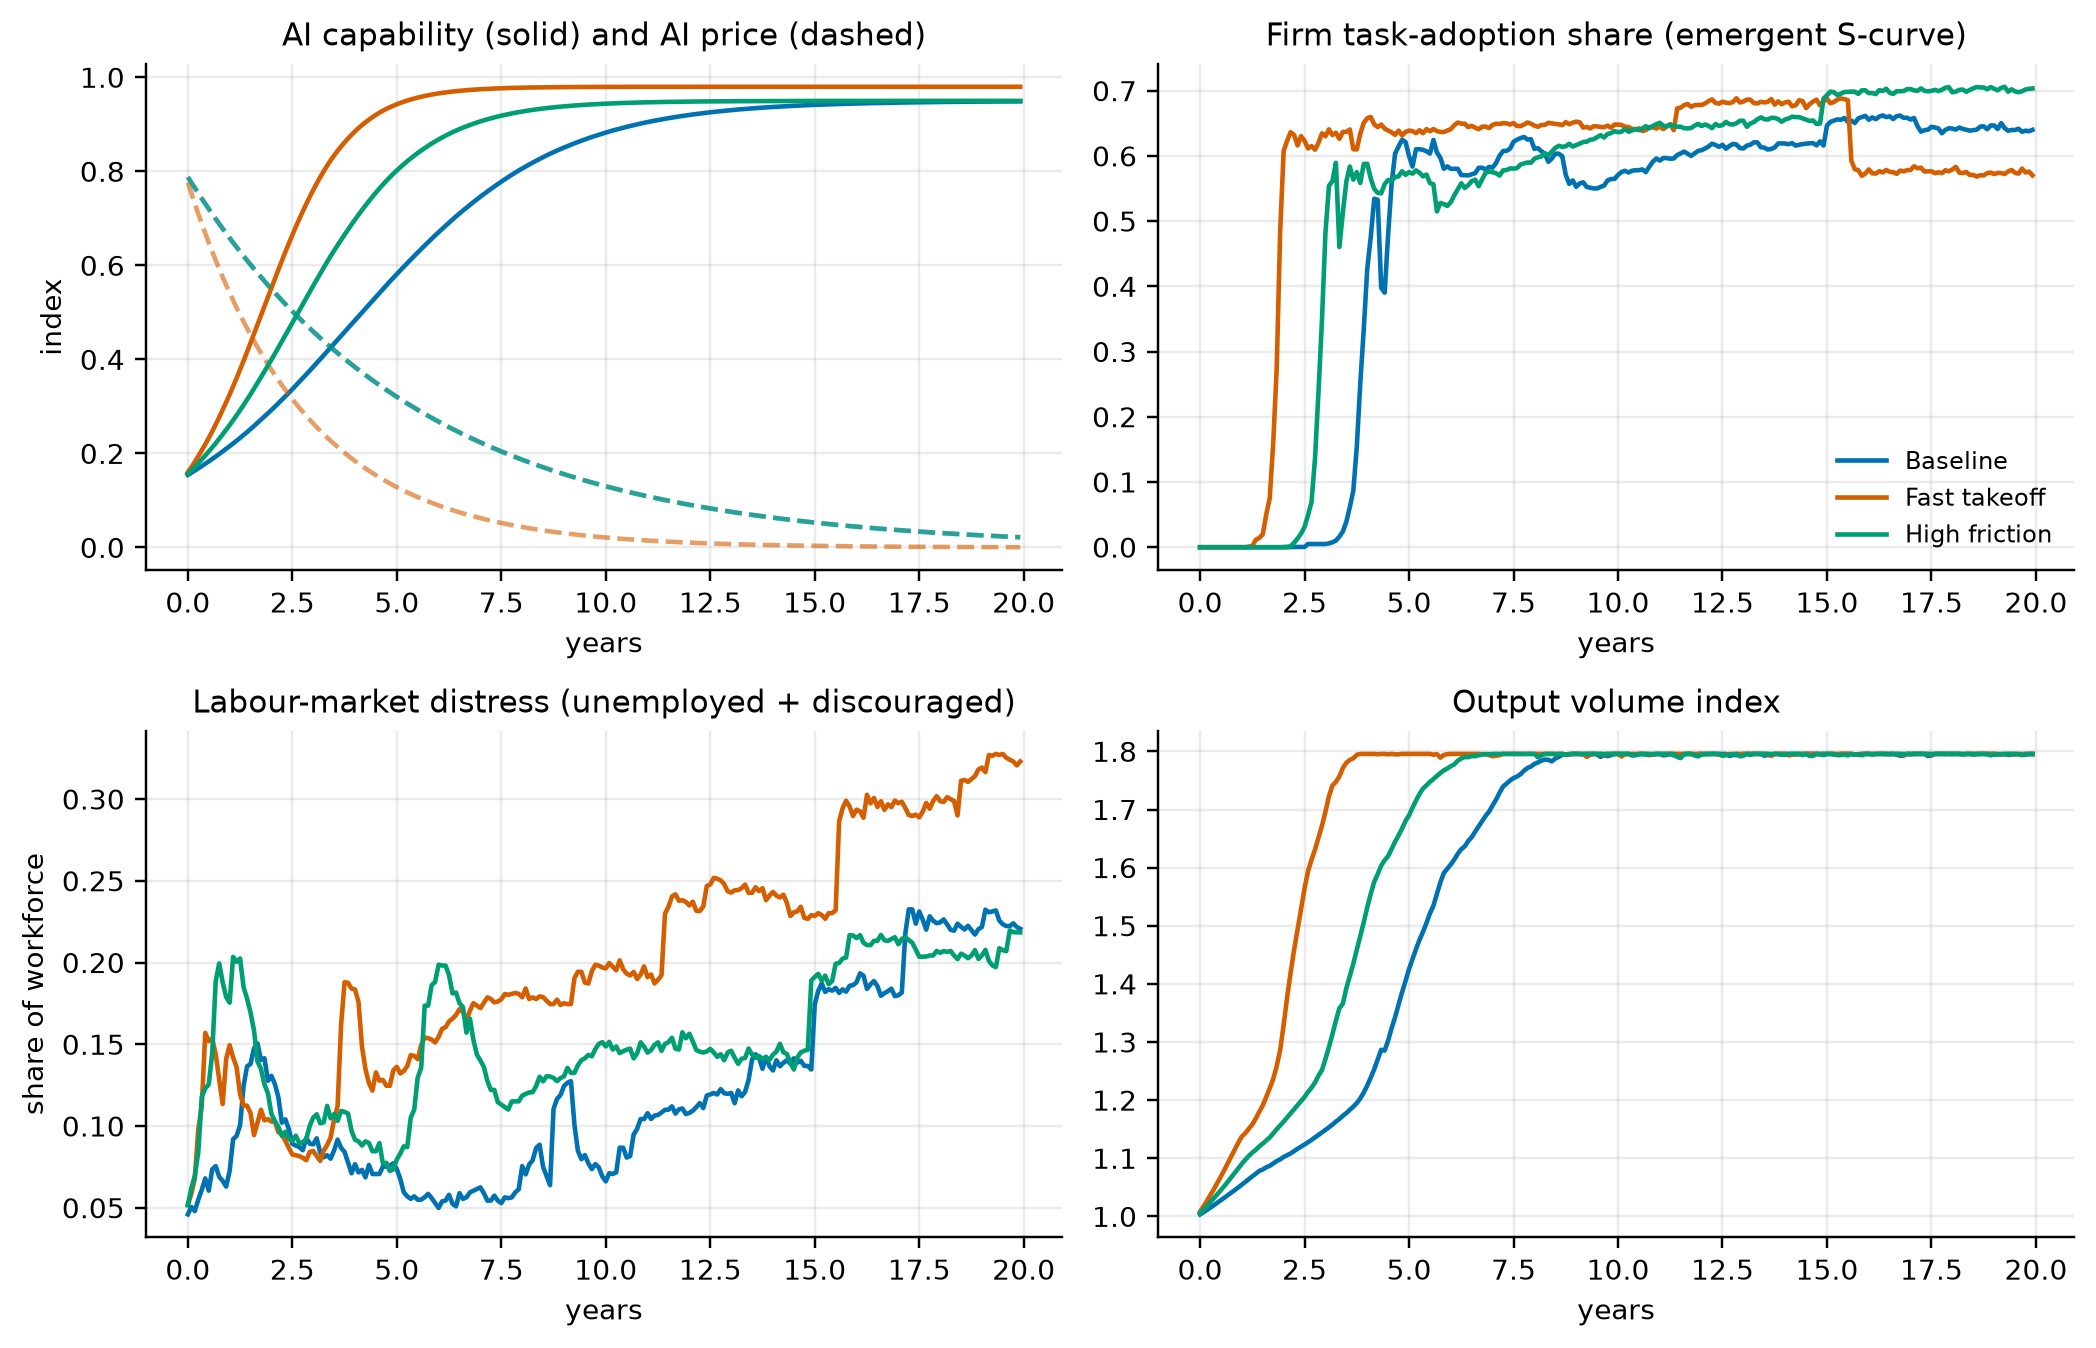
\includegraphics[width=0.92\textwidth]{figures/fig_scenarios.png}
\caption{Scenario comparison (seed 42, $N=2{,}000$, 20 years). Top left: capability
frontier (solid) and AI price (dashed). Top right: emergent adoption S-curves. Bottom:
labour-market distress and output. Nothing in the code imposes the S-shape.}
\label{fig:scenarios}
\end{figure}

\subsection{Uncertainty quantification}

Because tipping dynamics are nonlinear, single runs can mislead.
Figure~\ref{fig:montecarlo} shows percentile bands over 24 seeded replications of the
fast-takeoff scenario. The \emph{timing} of the adoption cascade is tightly
determined---it is driven by the capability process---but uncertainty grows along the
path: the median unemployment peak of roughly 16\% at the cascade spans about 14--20\%
across seeds, and by year twenty the p5--p95 band covers 11--23\% unemployment and
0.47--0.71 adoption, reflecting the path dependence of matching congestion and firm
exit cascades. Interquartile bands rather than single trajectories are therefore the
appropriate reporting unit for policy claims, and the application exposes them
directly.

\begin{figure}[t]
\centering
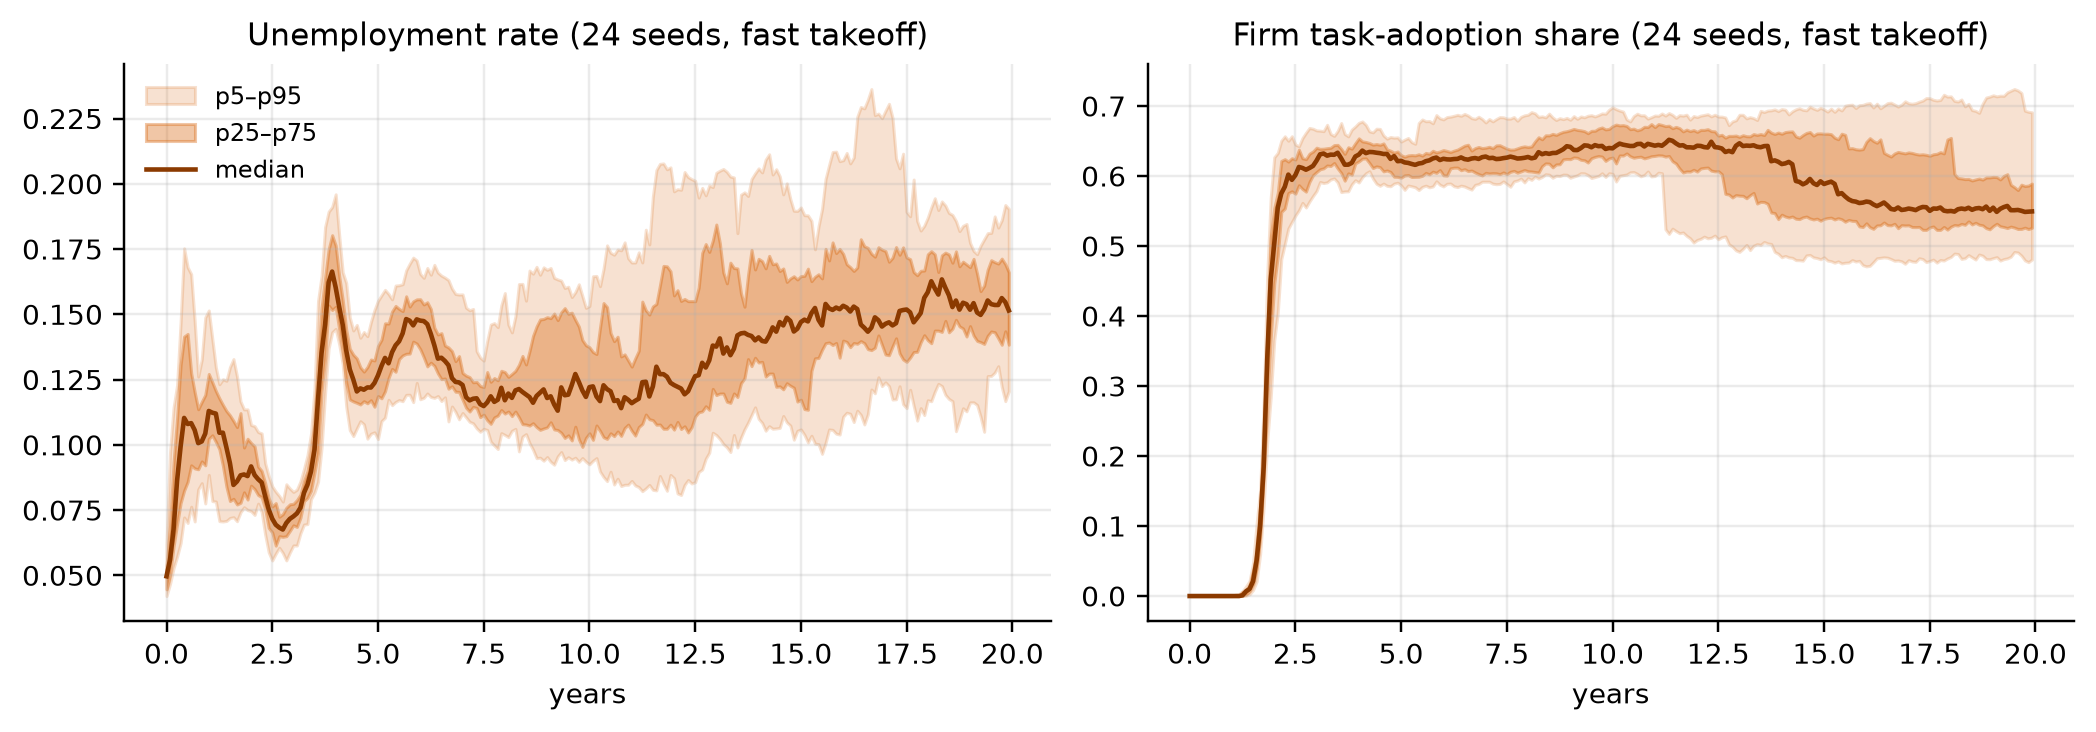
\includegraphics[width=0.92\textwidth]{figures/fig_montecarlo.png}
\caption{Monte Carlo uncertainty bands over 24 seeded replications (fast takeoff,
$N=1{,}500$). Shaded regions are p5--p95 and p25--p75; lines are medians.}
\label{fig:montecarlo}
\end{figure}

\subsection{Inequality and reallocation stress}

The left panel of Figure~\ref{fig:ineq} shows the wage-percentile fan under fast
takeoff, and the result is starker than a widening of dispersion: the median wage
roughly halves over the transition as automation reprices the marginal product of
exposed task mass across nearly all occupations, and displaced workers re-hired after
reservation-wage decay lock in persistent scars. Notably, the \emph{within-labour} Gini
drifts slightly \emph{down}---the wage distribution compresses toward the benefit floor
even as its level collapses. The model thus distinguishes two inequality concepts that
aggregate discussion often conflates: dispersion among workers falls while the implied
labour share of surplus (output nearly doubles as wages halve) shifts dramatically
toward firms and, in a richer model, capital owners. The right panel traces the
Beveridge curve. The no-AI baseline occupies a tight low-unemployment locus, while the
fast-takeoff economy sweeps through a two-phase loop: a vacancy-rich reallocation phase
during the adoption cascade, with vacancy rates transiently reaching tens of percent as
restructuring firms and entrants repost positions faster than the matching process can
fill them, followed by a slack regime far to the south-east where low vacancy rates
coexist with 10--19\% unemployment. This is the classic signature of
reallocation-driven mismatch \citep{blanchard1989beveridge}, generated here by the
distance structure of the occupation space rather than by an assumed mismatch index.

\begin{figure}[t]
\centering
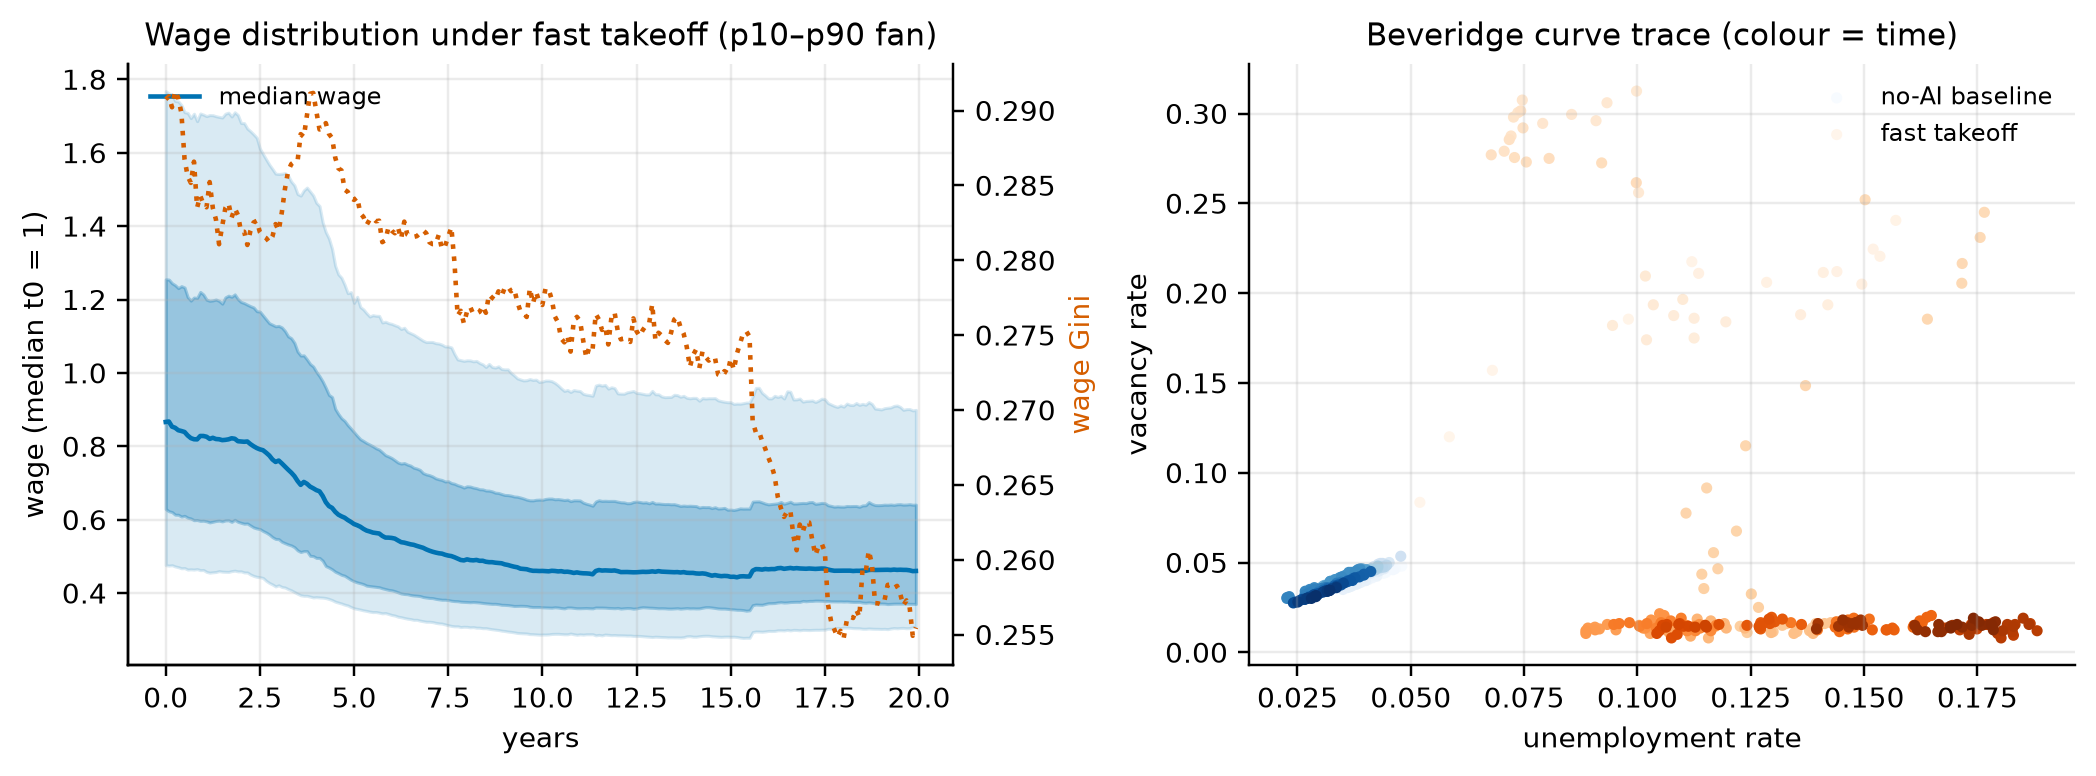
\includegraphics[width=0.92\textwidth]{figures/fig_inequality_beveridge.png}
\caption{Left: wage-percentile fan (p10--p90) and Gini under fast takeoff. Right:
Beveridge-curve traces for the no-AI baseline and fast takeoff; colour encodes time.}
\label{fig:ineq}
\end{figure}

\subsection{Policy experiments: non-robust levers}
\label{sec:policy}

Figure~\ref{fig:policy} reports peak distress across five seeds for three two-level
experiments under fast takeoff, and the headline finding is \emph{non-robustness} rather
than any single sign. Raising the benefit floor from 0.25 to 0.65 of the median wage
lowers median peak distress from 0.293 to 0.228---the income floor stabilizes
re-employment wages and keeps discouraged workers attached---yet two of five seeds
worsen, because the counteracting reservation-wage channel (generous benefits hold
reservation wages up exactly when re-employment requires accepting lower-paid work, the
classic moral-hazard margin of search theory, \citealp{pissarides2000equilibrium})
dominates on some tipping paths. Strikingly, an earlier development revision of the
product-market block produced the \emph{opposite} median ordering with the same
mechanisms present; the sign of the benefit effect is a property of the specification,
not of the model family. Raising firing costs from 0.05 to 0.60 leaves the median
essentially unchanged (0.240 vs.\ 0.234) while flipping sign seed-by-seed: employment
protection spreads displacement over time on some paths but delays it into a
synchronized, congested layoff wave on others. Only matching efficiency---the
throughput of the reallocation process itself---delivers a consistent median improvement
(0.226 fluid vs.\ 0.266 frictional), and it is the only monotonicity the test suite is
allowed to enforce; even here individual seeds deviate, so medians over replications,
not runs, are the unit of inference. We stress the epistemic status of these findings:
they are properties of a placeholder-calibrated model, valuable as hypothesis
generators and as a demonstration that an ABM can express---and expose---trade-offs and
specification risk that aggregate models bury in functional forms. Their ambiguity is
consistent with the mixed empirical evidence on labour-market programmes
\citep{card2018works}.

\begin{figure}[t]
\centering
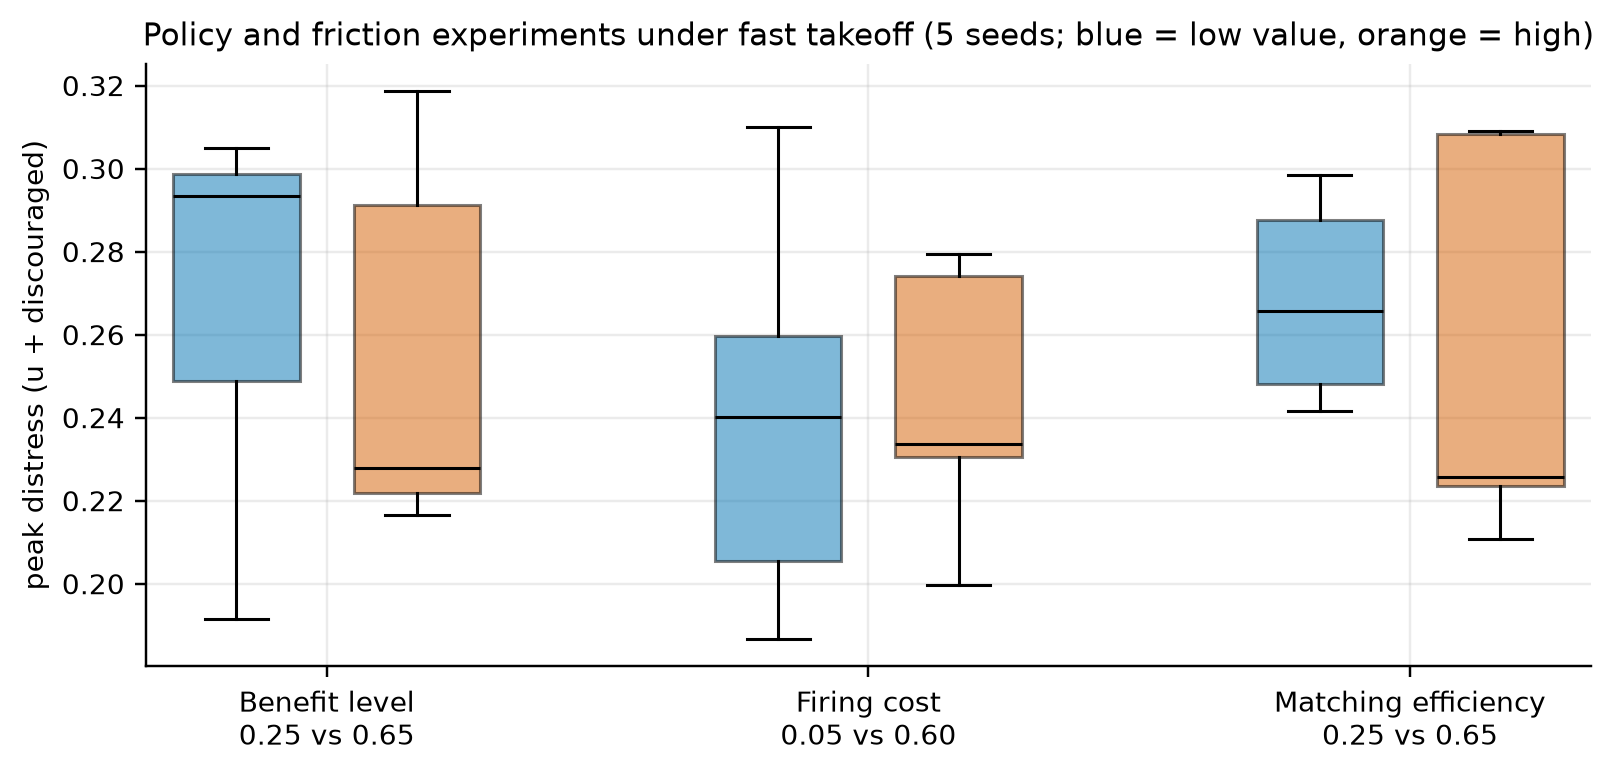
\includegraphics[width=0.78\textwidth]{figures/fig_policy.png}
\caption{Peak distress under fast takeoff across five seeds for three two-level
experiments (blue = low value, orange = high value). Benefits help in the median but
not in every seed; firing costs are a wash with seed-level sign flips; matching
efficiency delivers the only consistent median improvement.}
\label{fig:policy}
\end{figure}

Figure~\ref{fig:sweep} maps peak distress over the joint space of AI capability growth
and matching efficiency. The dominant feature is a threshold in speed: distress roughly
doubles between slow takeoff (2\% monthly capability growth, peak distress 0.09--0.13)
and moderate takeoff, and then approximately plateaus---once the adoption cascade
outruns the market's monthly reallocation capacity, additional speed adds little
further damage. Higher matching efficiency lowers distress across most of the grid,
most cleanly at slow and moderate speeds. At the fastest growth rates the two-seed cell
medians are visibly noisy, echoing the seed sensitivity of Section~\ref{sec:policy} and
motivating the denser replication proposed in Section~\ref{sec:future}.

\subsection{Organizational structure: the inverting pyramid}
\label{sec:pyramid}

Knowledge-intensive professional-service industries---consultancies, law firms,
engineering design, agencies---have historically organized as pyramids: a few partners
atop many mid-level and still more junior staff, with the junior layer serving both as
billable leverage and as the apprenticeship pipeline that produces future seniors.
Practitioner observation suggests AI-native firms in these sectors are emerging as
small \emph{inverted} pyramids: many senior experts exercising judgment, supported by
AI agents rather than junior staff. To test whether task-level economics alone can
generate this, we split five knowledge occupations (SOC 13, 15, 17, 23, 27) into
junior and senior variants: juniors carry the E2-heavy execution mass (research,
drafting, analysis, document review), seniors the judgment mass (negotiation,
strategy, supervision---E1 tasks with high difficulty and high augmentation), with
65/35 pyramid employment shares and a $\sim$2$\times$ senior wage premium. We also
sharpen the vintage effect: entrants now evaluate the \emph{entire} current technology
menu once at founding, so a new firm never builds the structure yesterday's technology
implied.

The task-level mechanism is sufficient for inversion, and brutally so
(Figure~\ref{fig:seniority}). Under fast takeoff, junior knowledge employment collapses
from 8\% of the workforce to zero within roughly five years---the five-seed median of
end-of-run junior employment is exactly zero---while senior employment persists
(median retention 1.01) as augmentation offsets the automation of seniors' residual
execution tasks. The pyramid ratio crosses inversion around year three and the junior
rung then ceases to exist: by the end of the run the senior--junior wage premium is not
large but \emph{undefined}, because there are no employed juniors left to compare.
Displaced juniors do not simply become seniors---four of the five junior--senior task
distances exceed the near-search radius, so the move requires the long-unemployment
retraining channel and its skill discount---they scatter across the wider occupation
space or into the unemployment and discouragement pools of Section~4.2.

The entrant/incumbent contrast, however, is largely \emph{not} reproduced, and the
failure is informative. AI-native entrants are directionally flatter during the cascade
(median junior staff share 0.49 vs.\ 0.53 for surviving $t_0$ incumbents), but the gap
is an order of magnitude smaller than the aggregate collapse, and both populations
converge to zero-junior structures within about two years of each other
(Figure~\ref{fig:seniority}, right). The reason is that the model's incumbents
re-optimize headcount targets monthly against weak adjustment frictions---they behave,
organizationally, like entrants with a legacy balance sheet. The stark
flat-entrant-beside-pyramidal-incumbent contrast observed in practice therefore cannot
be explained by differential technology access alone; within this framework it requires
multi-year organizational inertia in incumbents, an explicit apprenticeship production
function in which juniors are an investment in future seniors, or both. That
identification is Phase~A's most useful output: it converts a qualitative industry
observation into a measurement of organizational adjustment frictions, and it
motivates the promotion-channel extension of Section~\ref{sec:future}, where the
elimination of the junior rung should surface as a delayed senior-supply shortage
rather than today's quiet persistence.

\begin{figure}[t]
\centering
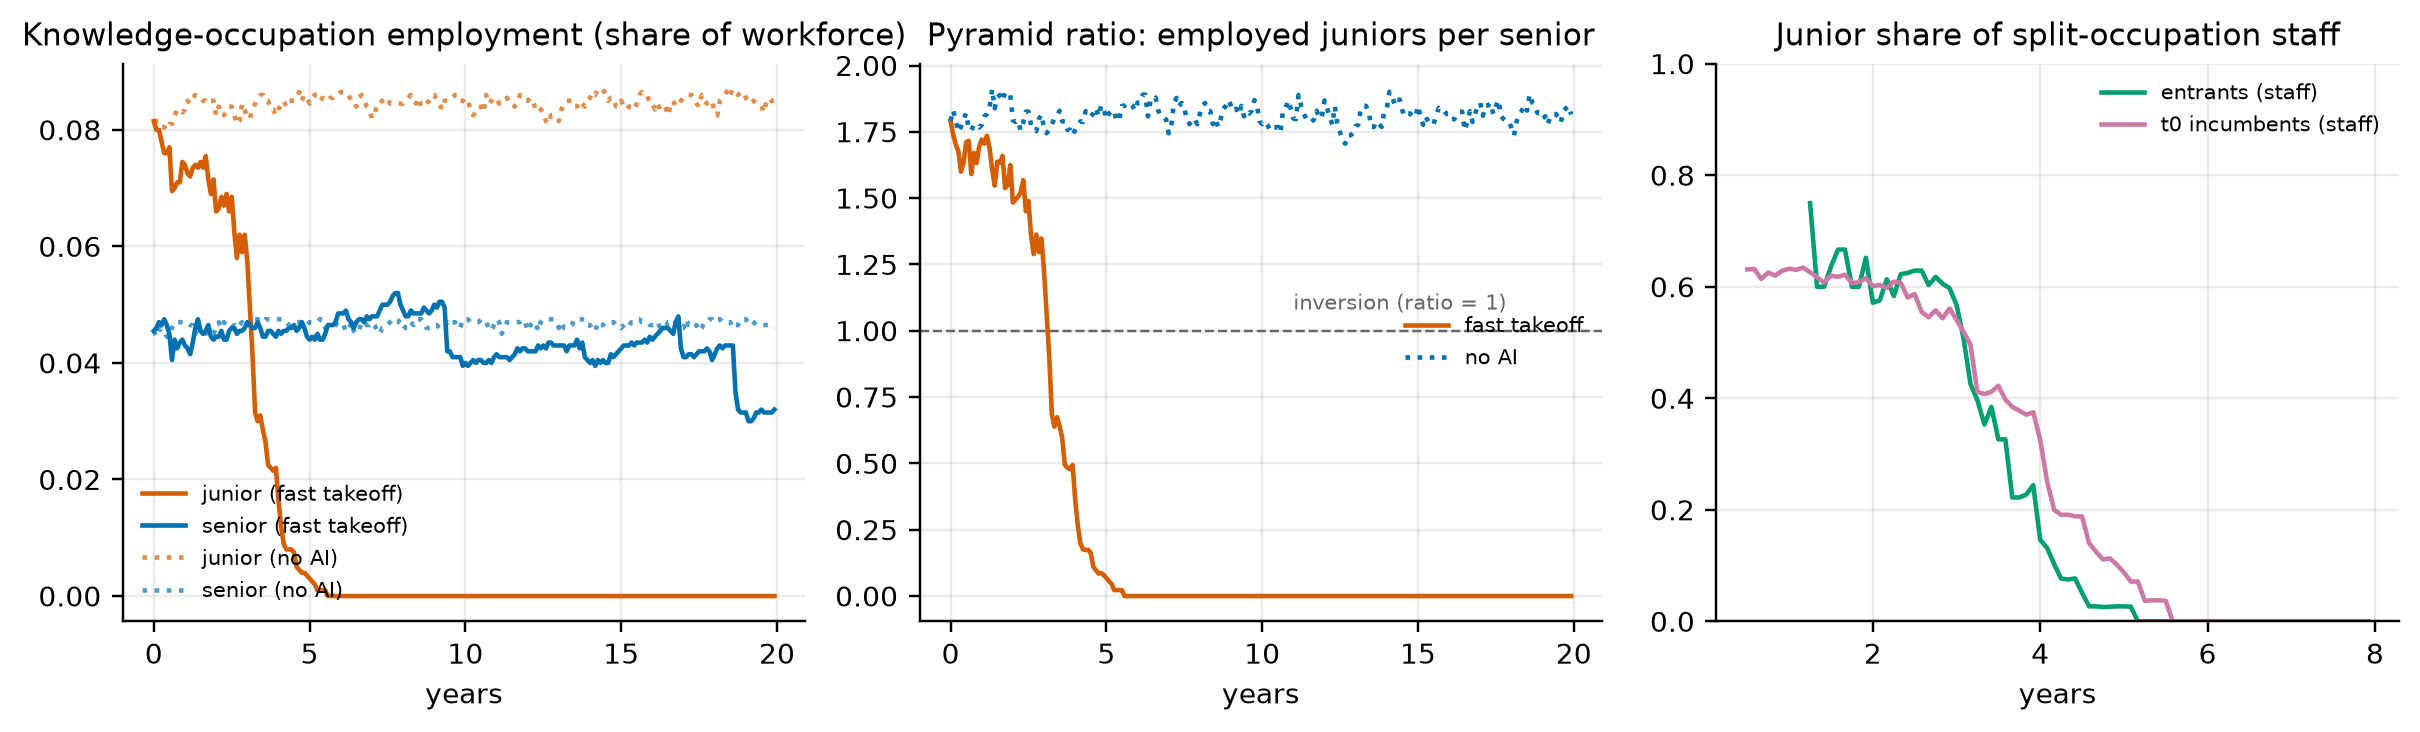
\includegraphics[width=\textwidth]{figures/fig_seniority.png}
\caption{The inverting pyramid (fast takeoff, seed 42, $N=2{,}000$; five-seed medians
in text). Left: junior knowledge employment collapses to zero while senior employment
persists; both are flat without AI. Centre: the junior:senior ratio crosses inversion
around year three. Right: AI-native entrants are only marginally flatter than
monthly-reoptimizing incumbents---the observed real-world contrast implies
organizational inertia the model does not yet contain.}
\label{fig:seniority}
\end{figure}

\begin{figure}[t]
\centering
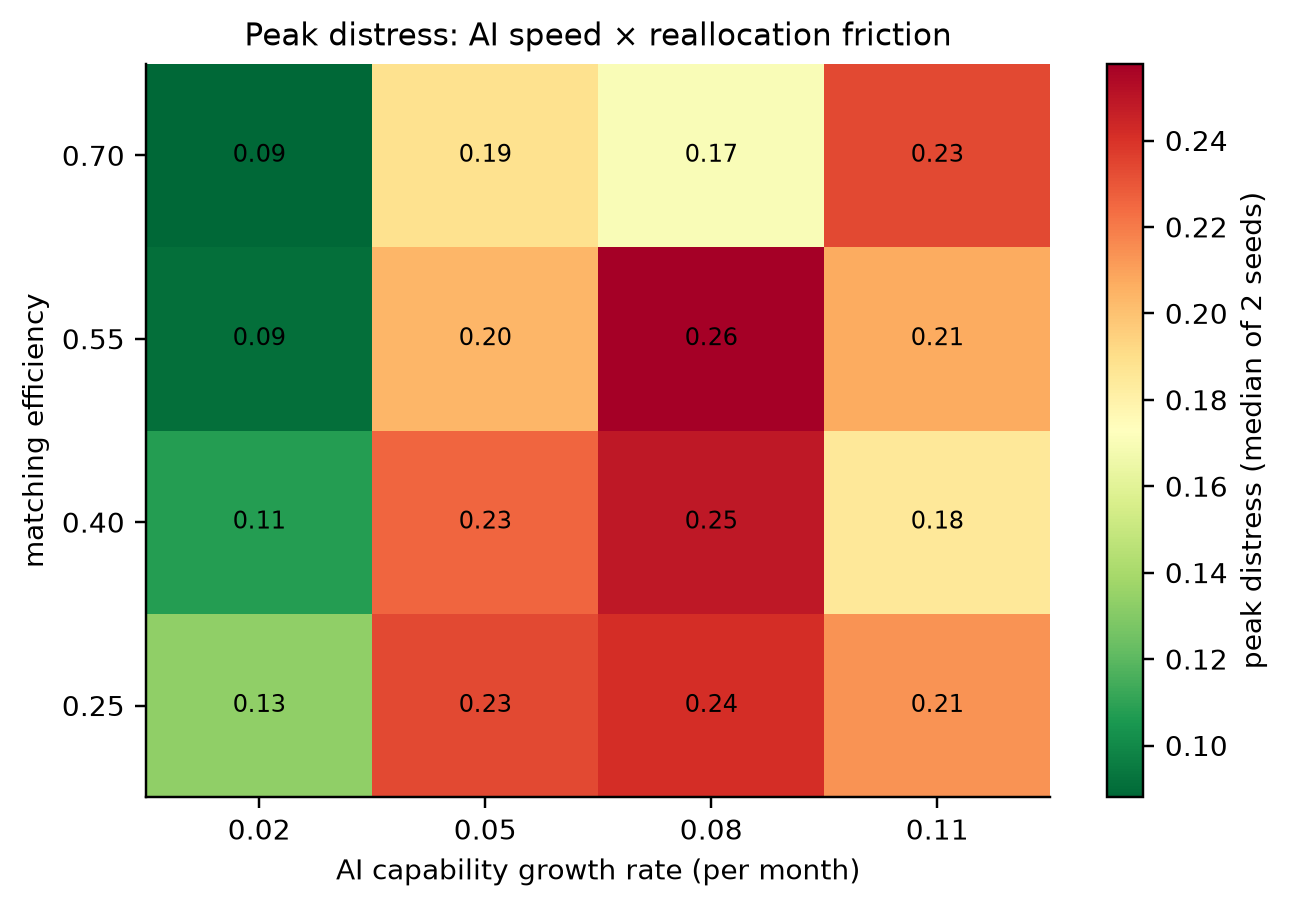
\includegraphics[width=0.55\textwidth]{figures/fig_sweep.png}
\caption{Peak distress over the AI-speed $\times$ reallocation-friction grid
(median of 2 seeds per cell, $N=800$, 12 years).}
\label{fig:sweep}
\end{figure}

\section{The interactive application}

The model ships as a two-page web application (Figure~\ref{fig:app}). The \emph{Live
model} page couples SolaraViz play/step/reset controls and parameter sliders to an
agent-space view in which workers appear as dots coloured by employment state,
clustered around employer firms drawn as squares sized by headcount and coloured by AI
adoption share; unemployed workers drift to a central ring. Time-series panels,
a wage-percentile fan, a Beveridge trace, an occupation-flow matrix, and CSV export
update each tick. The \emph{Research} page runs seeded Monte Carlo batches with live
progress, overlays two experiments' percentile bands, saves and loads versioned scenario
files, and executes one-dimensional parameter sweeps. The visual mode has proved
valuable for hypothesis generation---adoption cascades are literally visible as colour
fronts sweeping through sector clusters---while the batch mode supplies the statistical
discipline that single animated runs lack.

\begin{figure}[t]
\centering
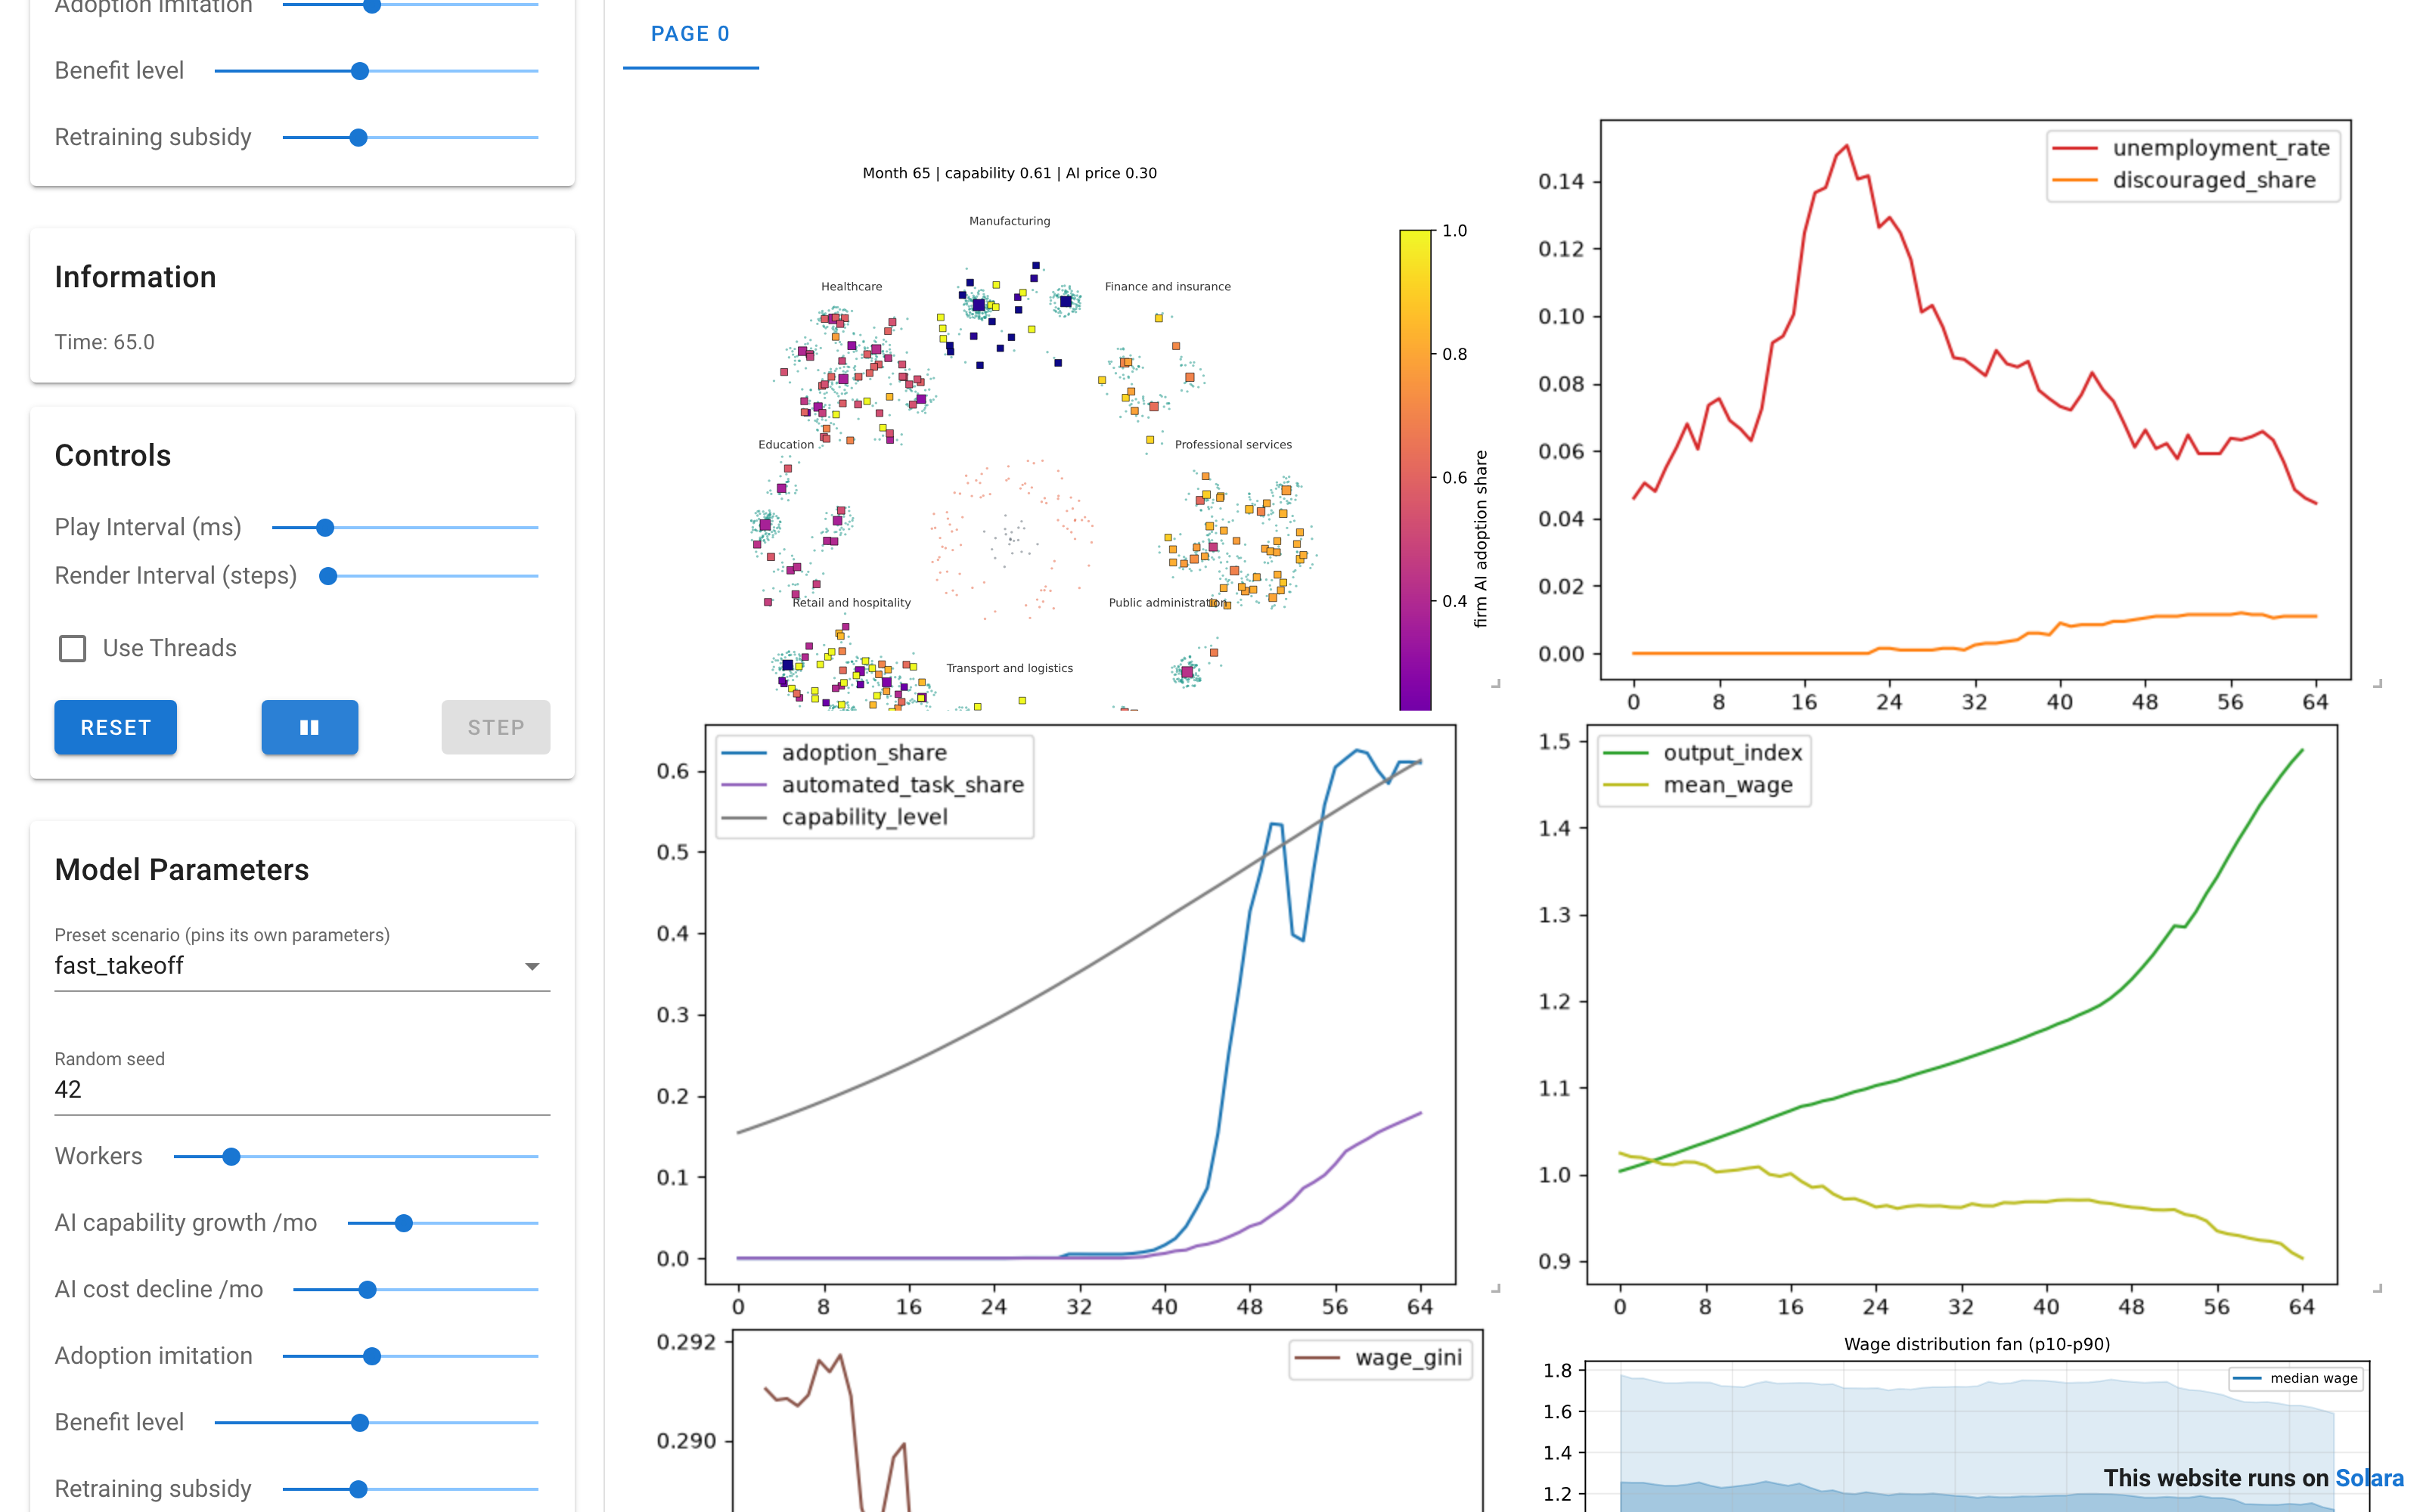
\includegraphics[width=0.47\textwidth]{figures/app_live.png}\hfill
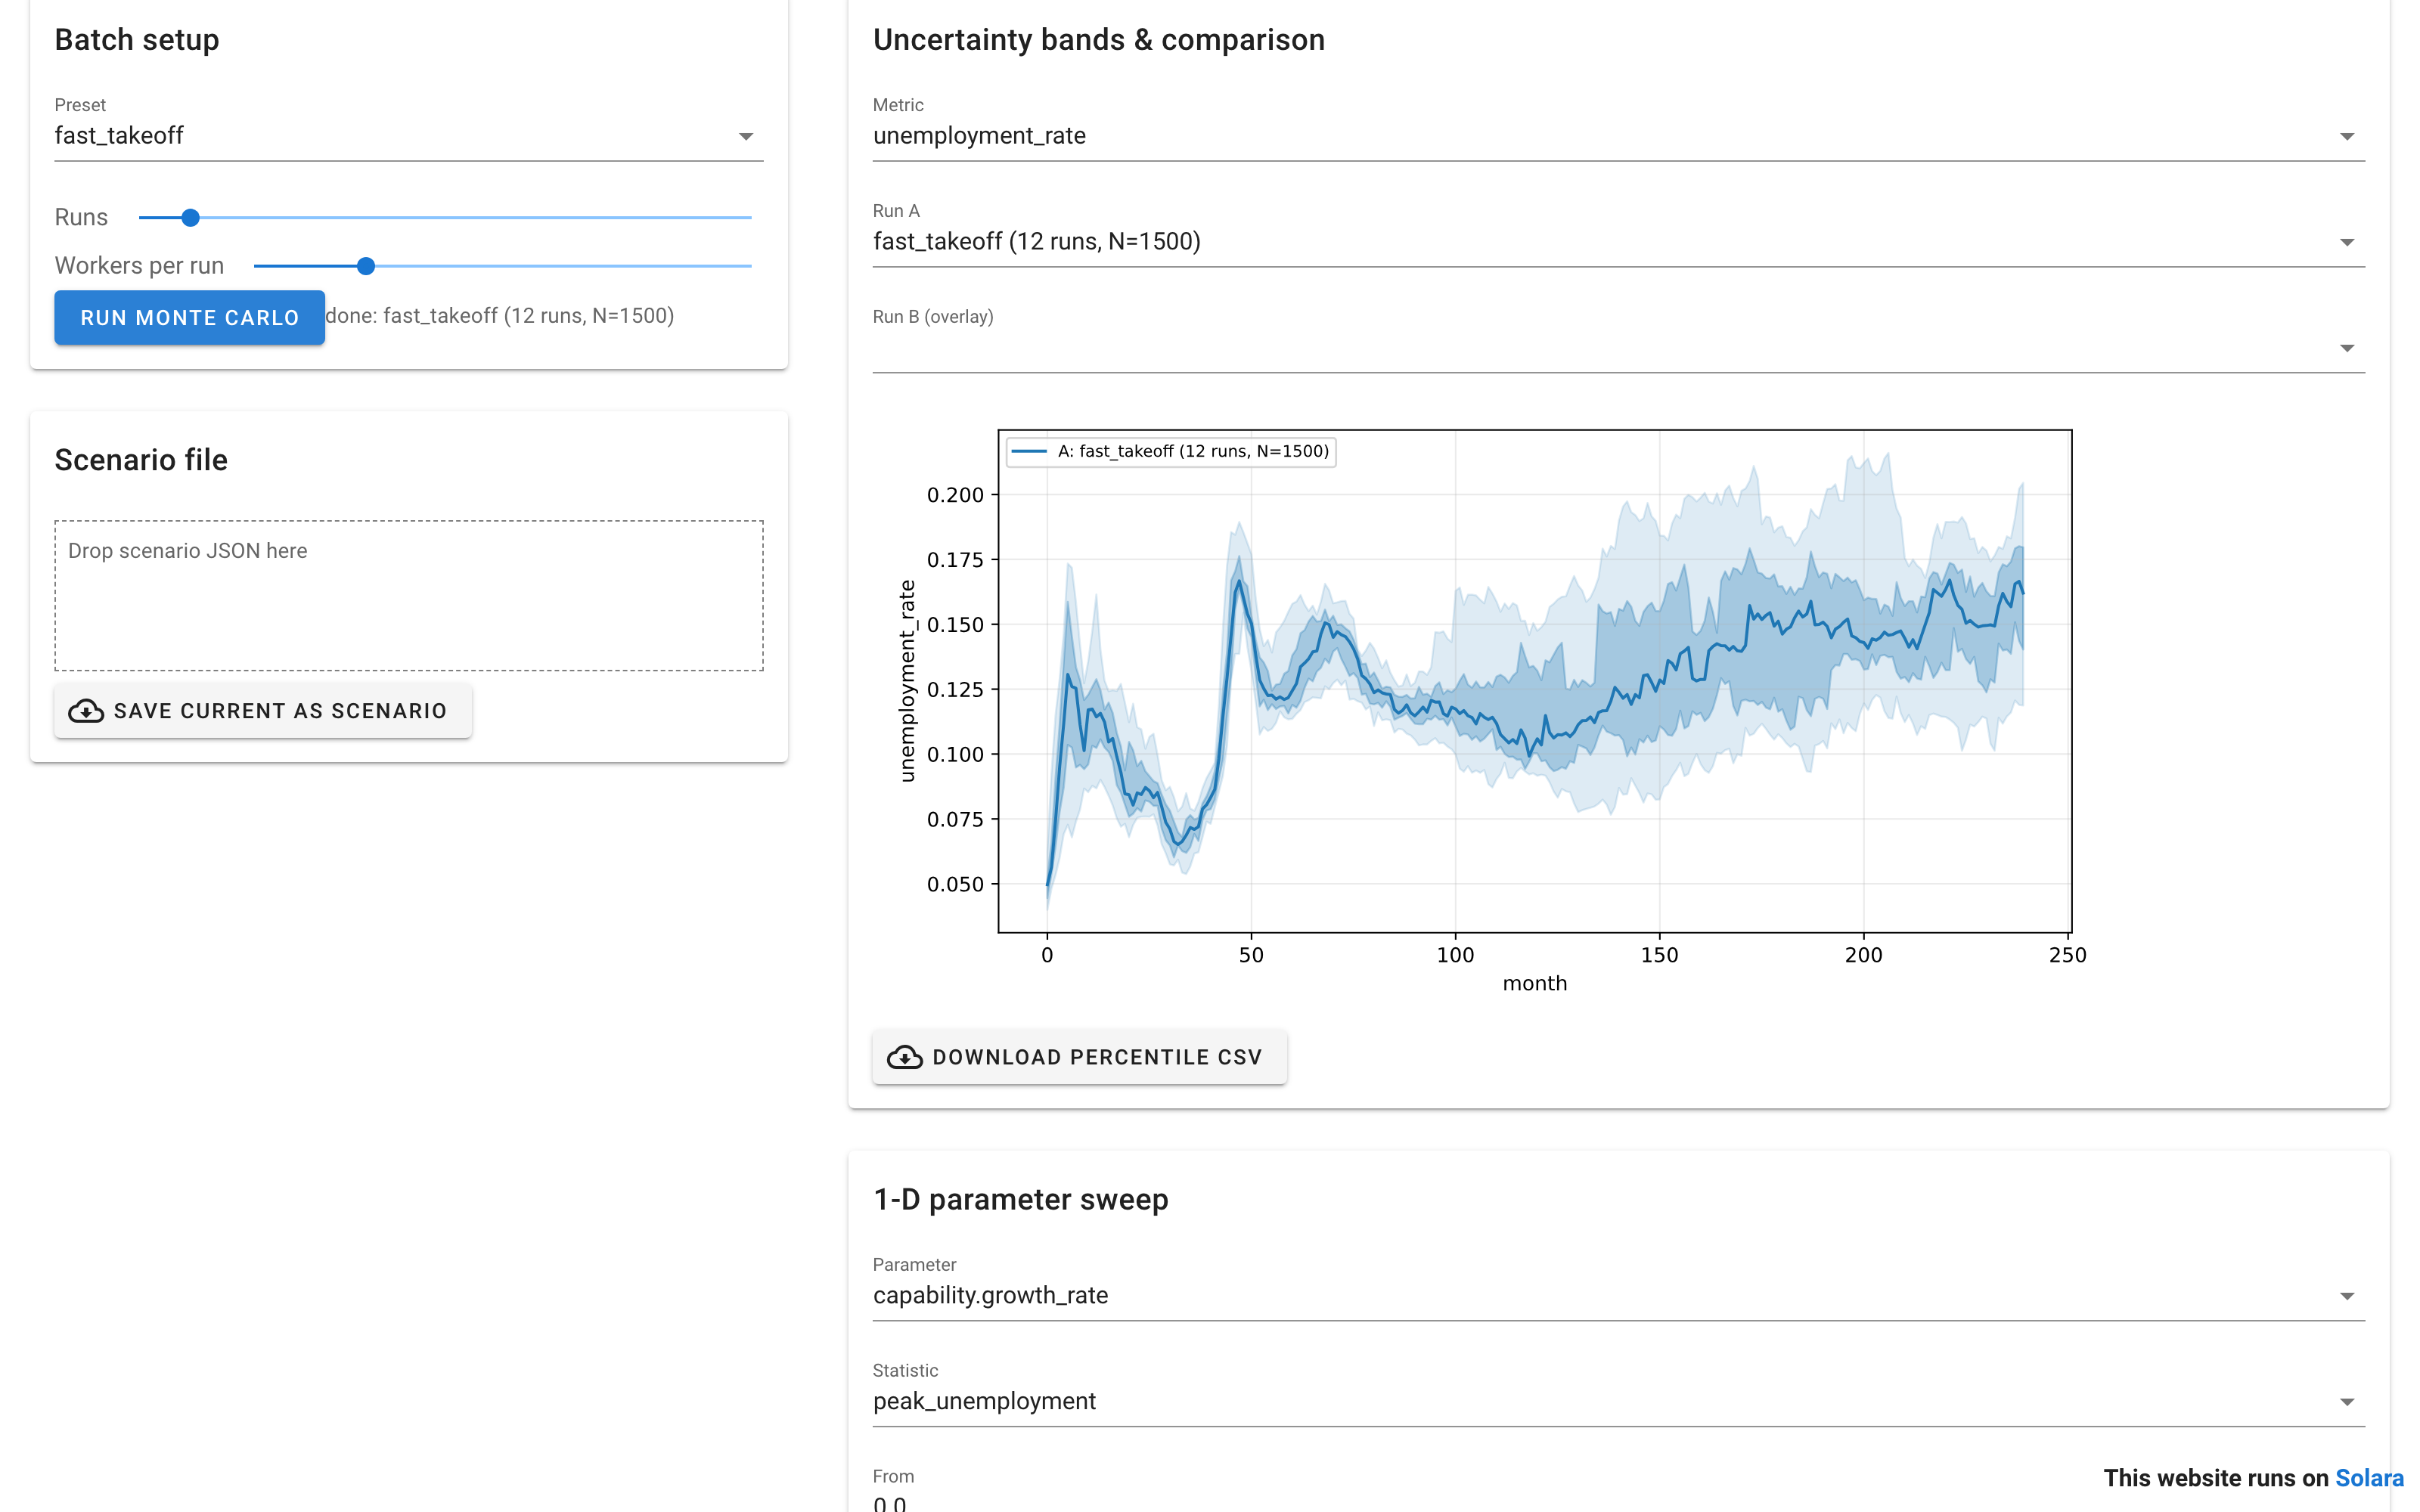
\includegraphics[width=0.47\textwidth]{figures/app_research.png}
\caption{The interactive application. Left: Live model page with agent-space view and
time-series panels. Right: Research page with Monte Carlo bands and parameter sweeps.}
\label{fig:app}
\end{figure}

\section{Discussion and limitations}

The exercise supports three methodological claims. First, the generative standard is
attainable at modest scale: a model small enough to audit line-by-line reproduces
S-curve diffusion, displacement-with-rebound, wage scarring, and Beveridge shifts from
first principles. Second, calibration gates---empirical anchor bands frozen as tests
before new mechanisms land---convert the folklore of ABM discipline
\citep{fagiolo2017macro, grimm2020odd} into an executable practice; each of the three
serious specification errors we made was caught by the gate, not by inspection. Third,
micro-founded policy analysis surfaces ambiguities that matter: the seed- and
specification-sensitivity of the benefit and firing-cost effects in
Section~\ref{sec:policy} would be invisible in a model whose transition path is a
dial---and a modeller who stopped at a single seed, or a single specification, would
have reported a confident sign that does not survive replication.

The sensitivities carry practical content of their own, because they tell decision-makers
\emph{where} confidence is and is not available. For policymakers, three implications
follow. Because the levers with the greatest political salience---benefit generosity and
employment protection---are exactly those whose effects proved fragile, transition policy
is better designed as an adaptive \emph{portfolio} (income support bundled with retraining
subsidies and matching investment, with pre-agreed adjustment triggers) than as a
commitment to any single instrument with an assumed sign. Guaranteed resources belong
instead with the one robustly signed lever, reallocation capacity: job-search assistance,
credential portability, and transparent skill taxonomies---the intervention class for
which empirical evidence is also least ambiguous \citep{card2018works}, and whose value
in the sweep is concentrated precisely in fast-takeoff regions where braking adoption
buys little beyond the congestion threshold. And because the cascade's \emph{timing} is
tightly determined even when its consequences are not
(Figure~\ref{fig:montecarlo}), monitoring dominates forecasting: adoption acceleration,
vacancy-to-searcher ratios, and Beveridge-curve displacement are observable precursors
that can arm state-contingent responses. A final measurement warning follows from
the inequality results (Figure~\ref{fig:ineq}): a regulator watching wage dispersion
alone would read the transition as equalizing while wage \emph{levels} collapse; the
labour share, not the within-labour Gini, is the statistic to track.

For managers the model reads as a survival analysis. The firm trait that most determines
exit during the transition is the idiosyncratic adoption hurdle---organizational
conservatism and evaluation capability---whose practical counterpart is a standing
discipline of task-level ROI review rather than episodic ``AI initiatives''; and because
complementarity operates \emph{within} occupations, that review must decompose jobs into
tasks, automating selectively and redesigning roles around the residual and augmented
bundle \citep{autor2015why}. Imitation dynamics imply that most firms restructure exactly
when their sector does, entering the labour market during the vacancy-rich mismatch phase
of the Beveridge loop; early movers hire and retrain at pre-cascade conditions, while
mid-cascade restructurers should expect long time-to-fill and treat retention of
task-adjacent staff as cheaper than search. The task-distance geometry doubles as an
internal redeployment map---mobility succeeds between task-adjacent roles and fails
across distant ones---and the seed-level variance of Figure~\ref{fig:montecarlo} argues
for staged, option-like AI investment over big-bang commitments, for the same reason the
policy conclusion favours triggers over fixed rules. Institutions that build monitoring,
adaptability, and reallocation capacity are robust to the model being wrong in either
direction; institutions optimized against one assumed transition path are fragile in
every direction but one.

The limitations are substantial and worth stating plainly. All task, occupation, and
sector parameters are placeholders; magnitudes (though not, we believe, mechanisms)
should be treated as illustrative. The model omits robotics (E0 tasks never automate),
aggregate-demand feedback from unemployment to consumption, capital markets, firm-level
AI implementation failures, within-occupation skill heterogeneity beyond a scalar, and
any geography. Discouragement and re-entry are stylized. Firms do not strategically
anticipate AI progress; adoption is myopic. Finally, a 24-task, 22-occupation grid is
coarse relative to the thousands of O*NET work activities.

\section{Future research and refinement}
\label{sec:future}

Five directions follow directly. \emph{First, empirical curation.} Replace placeholder
exposure, difficulty, and augmentation values with the published task-level estimates of
\citet{eloundou2024gpts} and observed usage intensities from \citet{handa2025economic};
weight occupations from O*NET work activities and BLS OES employment; validate the
implied occupation-distance matrix against observed occupational-transition matrices.
\emph{Second, mechanism extensions.} Add a robotics channel so E0 tasks automate on a
slower, capital-intensive schedule; endogenize task creation
\citep{acemoglu2019automation} so reinstatement competes with displacement; introduce
aggregate-demand feedback and firm balance sheets in the spirit of
\citet{dosi2010schumpeter}; let firms form expectations over the capability path. Most
immediately, Section~\ref{sec:pyramid} calls for a promotion channel (``Phase~B''):
senior vacancies restricted to workers with junior tenure, plus explicit organizational
adjustment inertia. Only then can the model price the apprenticeship
externality---individually rational junior cuts destroying the industry's future senior
supply---and reproduce the flat-entrant/pyramidal-incumbent contrast observed in
practice.
\emph{Third, deeper validation.} Confront the model with the emerging quasi-experimental
evidence on AI exposure and hiring \citep{hampole2025ai}, and test whether simulated
occupational wage responses match early observational estimates; historical automation
episodes (spreadsheets, industrial robots) offer out-of-sample transitions for
back-casting. \emph{Fourth, systematic exploration.} The seed-level variance visible in
Figure~\ref{fig:montecarlo} calls for global sensitivity analysis (e.g.\ Sobol indices
over the full parameter space) and for scaling tests confirming that results at
$N=5{,}000$ persist at $N=50{,}000$. \emph{Fifth, richer policy design.} The non-robust
single-lever results invite optimal-policy search over \emph{combinations}---benefit generosity
bundled with retraining subsidies and matching-technology investment---and evaluation of
timing rules that condition policy on observed adoption acceleration, a quantity the
model's tipping diagnostics already measure.

More broadly, the calibration-gate pattern and the derived-mobility-structure pattern
seem transferable to other technology-transition ABMs, and packaging them as reusable
methodology is itself a research contribution we intend to pursue.

{\small
\bibliographystyle{plainnat}
\bibliography{references}
}

\appendix

\section{Appendix: the model as a dependency graph}
\label{app:dependencies}

Figure~\ref{fig:dependencies} renders the model as a systems graph: every node is a
named mechanism from Section~3 (entities, the ten tick steps, policy parameters, and
outcome measures), and every directed edge is a ``reads from'' dependency stated
there---adoption ROI reads task quality, the AI price, and wages; headcount targets read
the demand factor, adoption, and augmentation; and so on. Node size reflects
connectivity. An interactive force-directed version with per-node documentation ships
with the repository (\texttt{docs/dependency-graph.html}); the node and edge lists are
maintained in \texttt{paper/dependency\_data.py}.

Four structural observations summarize how the model works and why it behaves as
reported. \emph{First, two hubs carry the system.} Task adoption is where the
technology block converges and from which the entire firm block fans out; job searchers
are where every displacement channel---layoffs, firm exits, exogenous
separations---pools before the matching bottleneck. These are the load-bearing joints,
and, not coincidentally, where the calibration gates caught all three serious
specification errors during development. \emph{Second, four feedback loops make
outcomes emergent rather than dial-driven}: the imitation loop (adoption
$\to$ peer imitation $\to$ adoption) is the cascade amplifier behind the S-curves of
Section~4.2; the demand-rebound loop (adoption $\to$ price $\to$ demand factor $\to$
headcount targets) is the job-preserving offset; the displacement--congestion loop
(layoffs $\to$ searchers $\to$ reservation wages $\to$ wages $\to$ adoption ROI) couples
labour-market slack back into adoption incentives; and the small discouragement cycle
governs labour-force attachment. \emph{Third, policy sits at the periphery}: each lever
touches exactly one edge of the densely cyclic core (firing costs $\to$ layoffs,
benefits $\to$ reservation wages, retraining subsidy $\to$ marginal product, matching
efficiency $\to$ matching). This is the graph-structural counterpart of
Section~\ref{sec:policy}'s non-robustness result---a single perturbed edge propagates
through whichever loop dominates a given stochastic path, so the sign of the net effect
is path-dependent. \emph{Fourth, the outcomes column has no outgoing edges}, and one
absent arrow is diagnostic: nothing feeds back from unemployment into product demand.
That missing aggregate-demand loop is the limitation flagged in Section~6 and the
demand-side extension proposed in Section~\ref{sec:future}.

\begin{figure}[t]
\centering
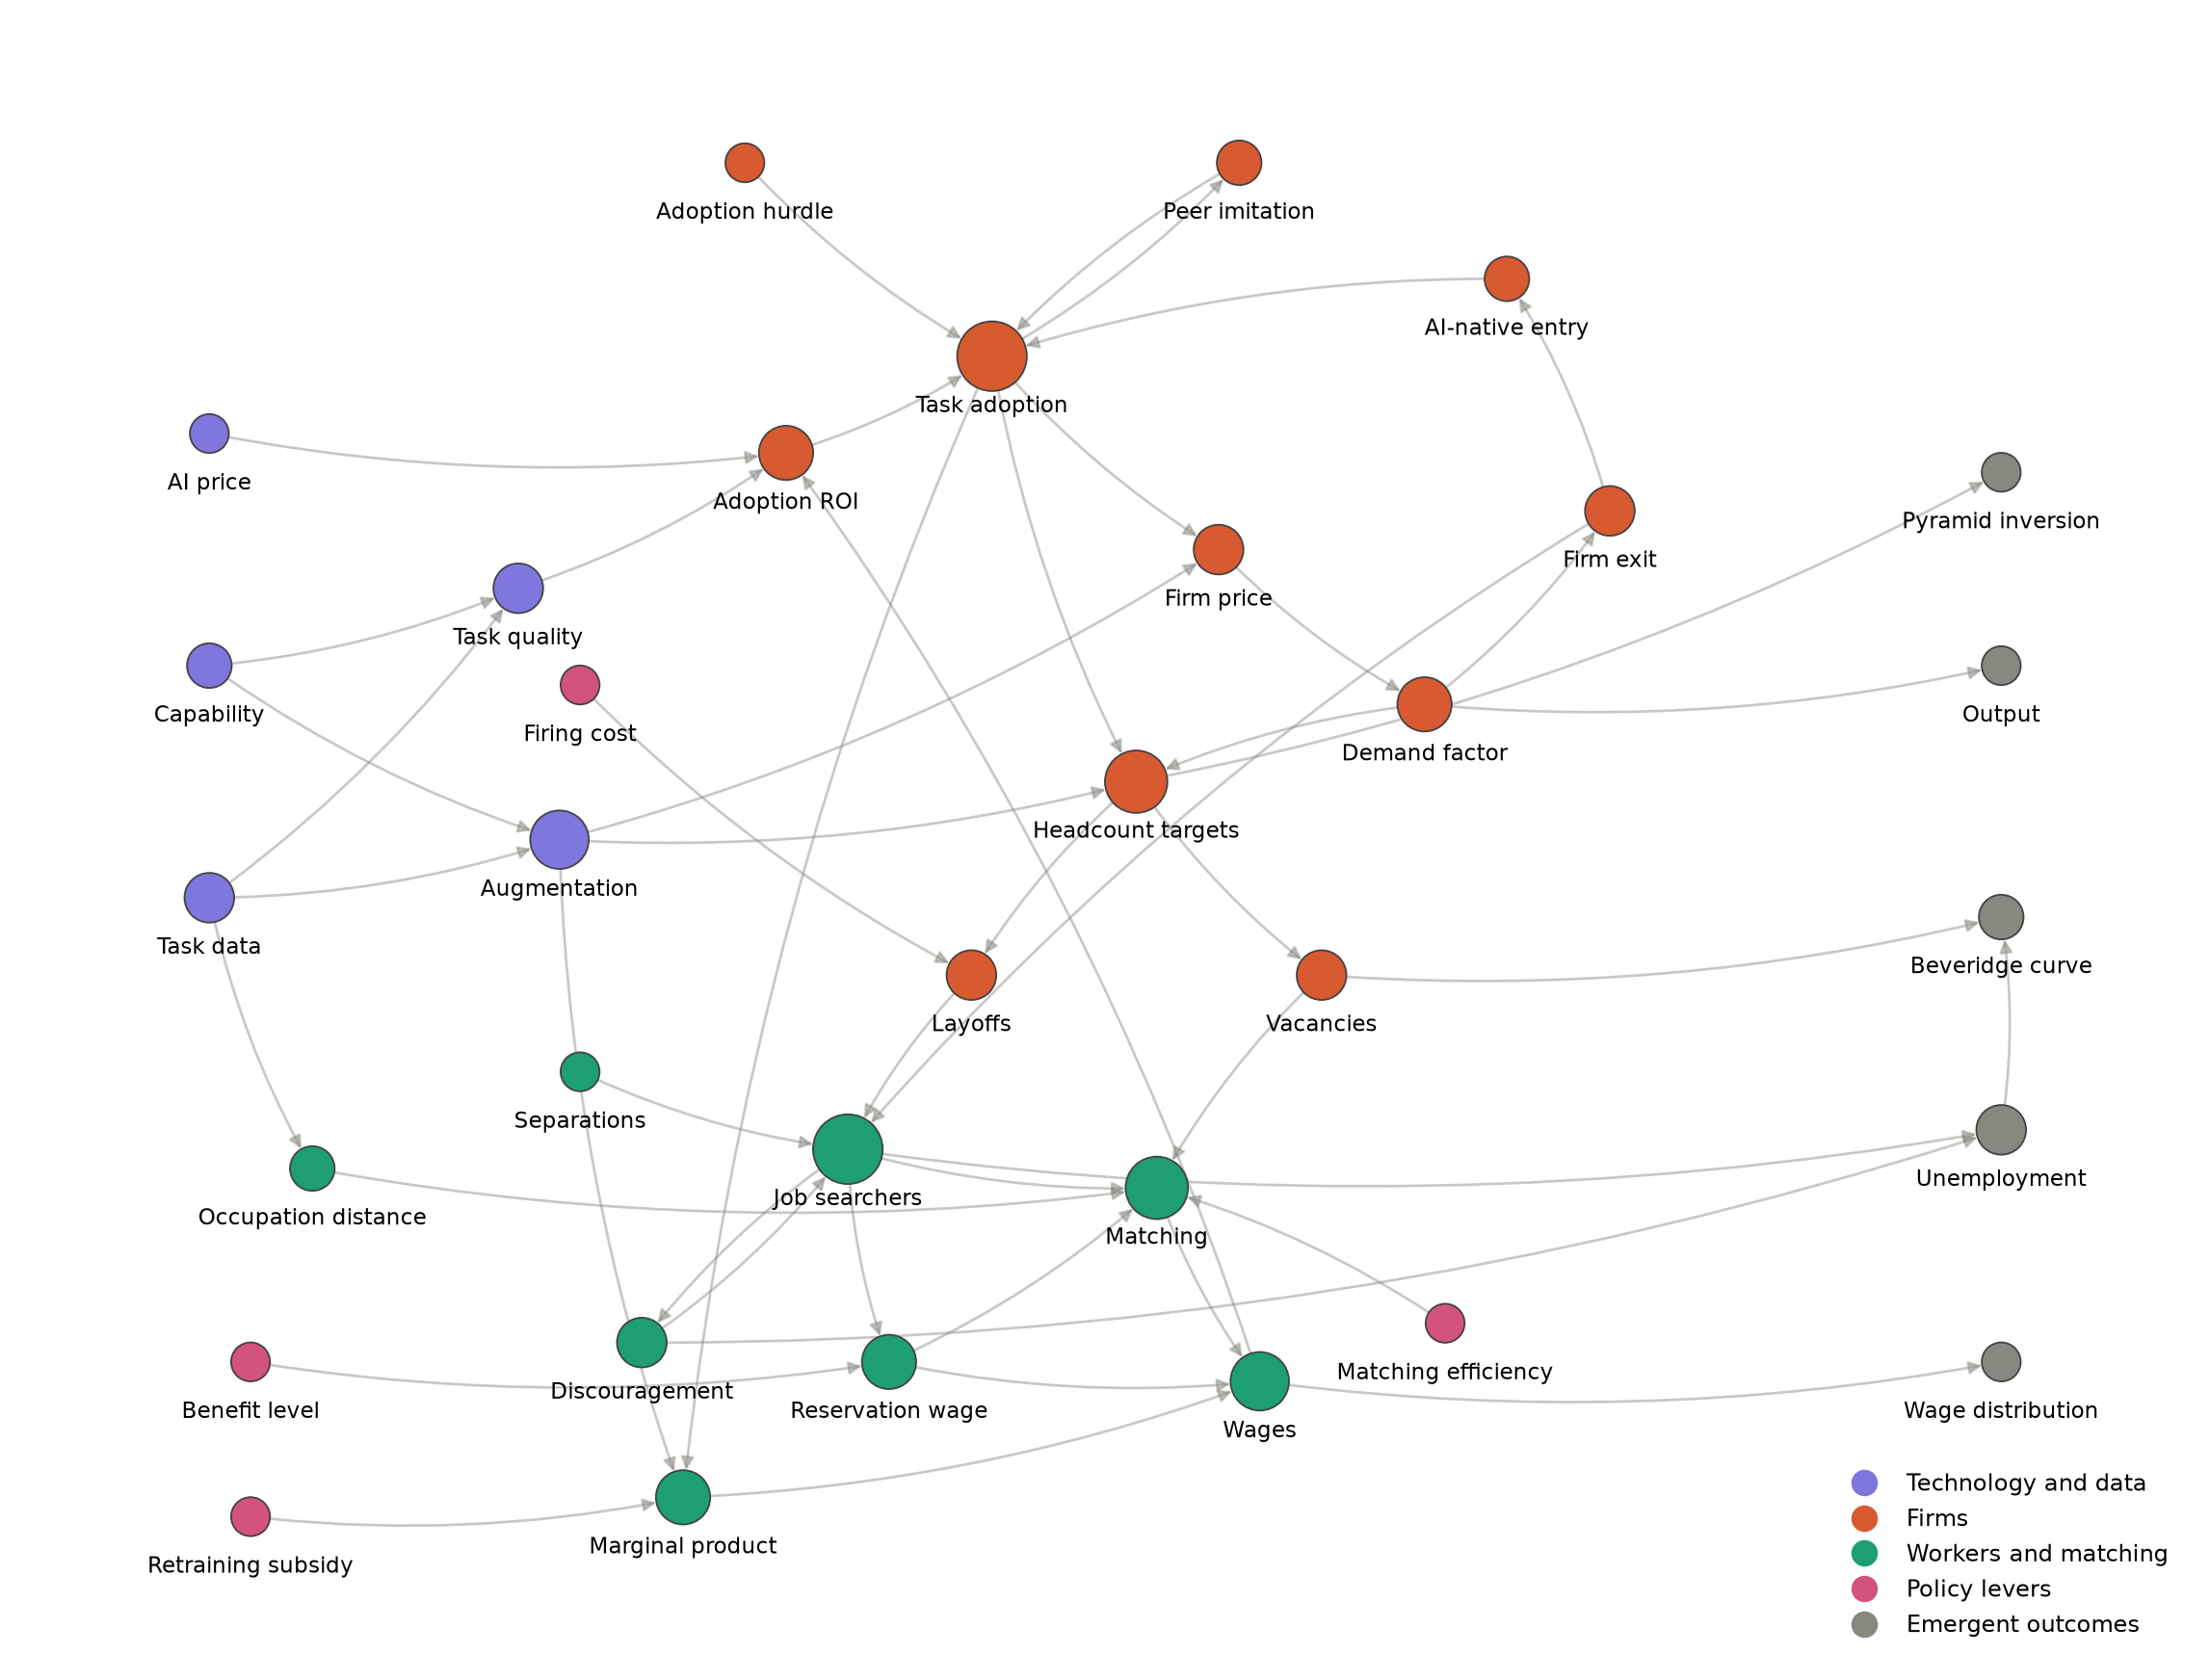
\includegraphics[width=\textwidth]{figures/fig_dependencies.png}
\caption{The simulation model as a dependency graph. Nodes are mechanisms, grouped and
coloured by subsystem; arrows point from a component to the components that read it;
node size reflects connectivity. Layout flows left to right from exogenous technology
and policy levers through the firm and labour-market blocks to emergent outcomes.}
\label{fig:dependencies}
\end{figure}



\end{document}
